\documentclass[]{article}
\usepackage{lmodern}
\usepackage{amssymb,amsmath}
\usepackage{ifxetex,ifluatex}
\usepackage{fixltx2e} % provides \textsubscript
\ifnum 0\ifxetex 1\fi\ifluatex 1\fi=0 % if pdftex
  \usepackage[T1]{fontenc}
  \usepackage[utf8]{inputenc}
\else % if luatex or xelatex
  \ifxetex
    \usepackage{mathspec}
    \usepackage{xltxtra,xunicode}
  \else
    \usepackage{fontspec}
  \fi
  \defaultfontfeatures{Mapping=tex-text,Scale=MatchLowercase}
  \newcommand{\euro}{€}
\fi
% use upquote if available, for straight quotes in verbatim environments
\IfFileExists{upquote.sty}{\usepackage{upquote}}{}
% use microtype if available
\IfFileExists{microtype.sty}{%
\usepackage{microtype}
\UseMicrotypeSet[protrusion]{basicmath} % disable protrusion for tt fonts
}{}
\usepackage[margin=1in]{geometry}
\usepackage{color}
\usepackage{fancyvrb}
\newcommand{\VerbBar}{|}
\newcommand{\VERB}{\Verb[commandchars=\\\{\}]}
\DefineVerbatimEnvironment{Highlighting}{Verbatim}{commandchars=\\\{\}}
% Add ',fontsize=\small' for more characters per line
\usepackage{framed}
\definecolor{shadecolor}{RGB}{248,248,248}
\newenvironment{Shaded}{\begin{snugshade}}{\end{snugshade}}
\newcommand{\KeywordTok}[1]{\textcolor[rgb]{0.13,0.29,0.53}{\textbf{{#1}}}}
\newcommand{\DataTypeTok}[1]{\textcolor[rgb]{0.13,0.29,0.53}{{#1}}}
\newcommand{\DecValTok}[1]{\textcolor[rgb]{0.00,0.00,0.81}{{#1}}}
\newcommand{\BaseNTok}[1]{\textcolor[rgb]{0.00,0.00,0.81}{{#1}}}
\newcommand{\FloatTok}[1]{\textcolor[rgb]{0.00,0.00,0.81}{{#1}}}
\newcommand{\CharTok}[1]{\textcolor[rgb]{0.31,0.60,0.02}{{#1}}}
\newcommand{\StringTok}[1]{\textcolor[rgb]{0.31,0.60,0.02}{{#1}}}
\newcommand{\CommentTok}[1]{\textcolor[rgb]{0.56,0.35,0.01}{\textit{{#1}}}}
\newcommand{\OtherTok}[1]{\textcolor[rgb]{0.56,0.35,0.01}{{#1}}}
\newcommand{\AlertTok}[1]{\textcolor[rgb]{0.94,0.16,0.16}{{#1}}}
\newcommand{\FunctionTok}[1]{\textcolor[rgb]{0.00,0.00,0.00}{{#1}}}
\newcommand{\RegionMarkerTok}[1]{{#1}}
\newcommand{\ErrorTok}[1]{\textbf{{#1}}}
\newcommand{\NormalTok}[1]{{#1}}
\usepackage{graphicx}
\makeatletter
\def\maxwidth{\ifdim\Gin@nat@width>\linewidth\linewidth\else\Gin@nat@width\fi}
\def\maxheight{\ifdim\Gin@nat@height>\textheight\textheight\else\Gin@nat@height\fi}
\makeatother
% Scale images if necessary, so that they will not overflow the page
% margins by default, and it is still possible to overwrite the defaults
% using explicit options in \includegraphics[width, height, ...]{}
\setkeys{Gin}{width=\maxwidth,height=\maxheight,keepaspectratio}
\ifxetex
  \usepackage[setpagesize=false, % page size defined by xetex
              unicode=false, % unicode breaks when used with xetex
              xetex]{hyperref}
\else
  \usepackage[unicode=true]{hyperref}
\fi
\hypersetup{breaklinks=true,
            bookmarks=true,
            pdfauthor={Zanin Pavel},
            pdftitle={Reproducible-Research---Course-Project-2},
            colorlinks=true,
            citecolor=blue,
            urlcolor=blue,
            linkcolor=magenta,
            pdfborder={0 0 0}}
\urlstyle{same}  % don't use monospace font for urls
\setlength{\parindent}{0pt}
\setlength{\parskip}{6pt plus 2pt minus 1pt}
\setlength{\emergencystretch}{3em}  % prevent overfull lines
\setcounter{secnumdepth}{0}

%%% Use protect on footnotes to avoid problems with footnotes in titles
\let\rmarkdownfootnote\footnote%
\def\footnote{\protect\rmarkdownfootnote}

%%% Change title format to be more compact
\usepackage{titling}

% Create subtitle command for use in maketitle
\newcommand{\subtitle}[1]{
  \posttitle{
    \begin{center}\large#1\end{center}
    }
}

\setlength{\droptitle}{-2em}
  \title{Reproducible-Research---Course-Project-2}
  \pretitle{\vspace{\droptitle}\centering\huge}
  \posttitle{\par}
  \author{Zanin Pavel}
  \preauthor{\centering\large\emph}
  \postauthor{\par}
  \predate{\centering\large\emph}
  \postdate{\par}
  \date{February 29, 2016}



\begin{document}

\maketitle


\section{Synopsis}\label{synopsis}

This project involves exploring the U.S. National Oceanic and
Atmospheric Administration's (NOAA) storm database. This database tracks
characteristics of major storms and weather events in the United States,
including when and where they occur, as well as estimates of any
fatalities, injuries, and property damage.

\textbf{Data}

The data for this assignment come in the form of a comma-separated-value
file compressed via the bzip2 algorithm to reduce its size. You can find
file in
\href{https://github.com/Filareth2015/Reproducible-Research---Course-Project-2}{course
work project folder class} .

There is also some documentation of the database available. Here you
will find how some of the variables are constructed/defined.

\begin{itemize}
\itemsep1pt\parskip0pt\parsep0pt
\item
  National Weather Service Storm Data Documentation
  \href{https://github.com/Filareth2015/Reproducible-Research---Course-Project-2}{see}\\
\item
  National Climatic Data Center Storm Events FAQ
  \href{https://github.com/Filareth2015/Reproducible-Research---Course-Project-2}{see}
\end{itemize}

The events in the database start in the year 1950 and end in November
2011. In the earlier years of the database there are generally fewer
events recorded, most likely due to a lack of good records. More recent
years should be considered more complete.

\textbf{Assignment}

The basic goal of this assignment is to explore the NOAA Storm Database
and answer some basic questions about severe weather events. You must
use the database to answer the questions below and show the code for
your entire analysis. Your analysis can consist of tables, figures, or
other summaries. You may use any R package you want to support your
analysis.

\textbf{Questions}

Your data analysis must address the following questions:

\begin{enumerate}
\def\labelenumi{\arabic{enumi}.}
\itemsep1pt\parskip0pt\parsep0pt
\item
  Across the United States, which types of events (as indicated in the
  EVTYPE variable) are most harmful with respect to population health?
\item
  Across the United States, which types of events have the greatest
  economic consequences?
\end{enumerate}

Consider writing your report as if it were to be read by a government or
municipal manager who might be responsible for preparing for severe
weather events and will need to prioritize resources for different types
of events. However, there is no need to make any specific
recommendations in your report.

\section{1. Data Processing}\label{data-processing}

Loading the data.

\begin{Shaded}
\begin{Highlighting}[]
\NormalTok{storm.data =}\StringTok{ }\KeywordTok{read.csv}\NormalTok{(}\KeywordTok{bzfile}\NormalTok{(}\StringTok{"repdata-data-StormData.csv.bz2"}\NormalTok{), }\DataTypeTok{header =} \OtherTok{TRUE}\NormalTok{)}
\end{Highlighting}
\end{Shaded}

Loaded data's summary:

\begin{Shaded}
\begin{Highlighting}[]
\KeywordTok{str}\NormalTok{(storm.data)}
\end{Highlighting}
\end{Shaded}

\begin{verbatim}
## 'data.frame':    902297 obs. of  37 variables:
##  $ STATE__   : num  1 1 1 1 1 1 1 1 1 1 ...
##  $ BGN_DATE  : Factor w/ 16335 levels "1/1/1966 0:00:00",..: 6523 6523 4242 11116 2224 2224 2260 383 3980 3980 ...
##  $ BGN_TIME  : Factor w/ 3608 levels "00:00:00 AM",..: 272 287 2705 1683 2584 3186 242 1683 3186 3186 ...
##  $ TIME_ZONE : Factor w/ 22 levels "ADT","AKS","AST",..: 7 7 7 7 7 7 7 7 7 7 ...
##  $ COUNTY    : num  97 3 57 89 43 77 9 123 125 57 ...
##  $ COUNTYNAME: Factor w/ 29601 levels "","5NM E OF MACKINAC BRIDGE TO PRESQUE ISLE LT MI",..: 13513 1873 4598 10592 4372 10094 1973 23873 24418 4598 ...
##  $ STATE     : Factor w/ 72 levels "AK","AL","AM",..: 2 2 2 2 2 2 2 2 2 2 ...
##  $ EVTYPE    : Factor w/ 985 levels "   HIGH SURF ADVISORY",..: 834 834 834 834 834 834 834 834 834 834 ...
##  $ BGN_RANGE : num  0 0 0 0 0 0 0 0 0 0 ...
##  $ BGN_AZI   : Factor w/ 35 levels "","  N"," NW",..: 1 1 1 1 1 1 1 1 1 1 ...
##  $ BGN_LOCATI: Factor w/ 54429 levels "","- 1 N Albion",..: 1 1 1 1 1 1 1 1 1 1 ...
##  $ END_DATE  : Factor w/ 6663 levels "","1/1/1993 0:00:00",..: 1 1 1 1 1 1 1 1 1 1 ...
##  $ END_TIME  : Factor w/ 3647 levels ""," 0900CST",..: 1 1 1 1 1 1 1 1 1 1 ...
##  $ COUNTY_END: num  0 0 0 0 0 0 0 0 0 0 ...
##  $ COUNTYENDN: logi  NA NA NA NA NA NA ...
##  $ END_RANGE : num  0 0 0 0 0 0 0 0 0 0 ...
##  $ END_AZI   : Factor w/ 24 levels "","E","ENE","ESE",..: 1 1 1 1 1 1 1 1 1 1 ...
##  $ END_LOCATI: Factor w/ 34506 levels "","- .5 NNW",..: 1 1 1 1 1 1 1 1 1 1 ...
##  $ LENGTH    : num  14 2 0.1 0 0 1.5 1.5 0 3.3 2.3 ...
##  $ WIDTH     : num  100 150 123 100 150 177 33 33 100 100 ...
##  $ F         : int  3 2 2 2 2 2 2 1 3 3 ...
##  $ MAG       : num  0 0 0 0 0 0 0 0 0 0 ...
##  $ FATALITIES: num  0 0 0 0 0 0 0 0 1 0 ...
##  $ INJURIES  : num  15 0 2 2 2 6 1 0 14 0 ...
##  $ PROPDMG   : num  25 2.5 25 2.5 2.5 2.5 2.5 2.5 25 25 ...
##  $ PROPDMGEXP: Factor w/ 19 levels "","-","?","+",..: 17 17 17 17 17 17 17 17 17 17 ...
##  $ CROPDMG   : num  0 0 0 0 0 0 0 0 0 0 ...
##  $ CROPDMGEXP: Factor w/ 9 levels "","?","0","2",..: 1 1 1 1 1 1 1 1 1 1 ...
##  $ WFO       : Factor w/ 542 levels ""," CI","$AC",..: 1 1 1 1 1 1 1 1 1 1 ...
##  $ STATEOFFIC: Factor w/ 250 levels "","ALABAMA, Central",..: 1 1 1 1 1 1 1 1 1 1 ...
##  $ ZONENAMES : Factor w/ 25112 levels "","                                                                                                                               "| __truncated__,..: 1 1 1 1 1 1 1 1 1 1 ...
##  $ LATITUDE  : num  3040 3042 3340 3458 3412 ...
##  $ LONGITUDE : num  8812 8755 8742 8626 8642 ...
##  $ LATITUDE_E: num  3051 0 0 0 0 ...
##  $ LONGITUDE_: num  8806 0 0 0 0 ...
##  $ REMARKS   : Factor w/ 436781 levels "","-2 at Deer Park\n",..: 1 1 1 1 1 1 1 1 1 1 ...
##  $ REFNUM    : num  1 2 3 4 5 6 7 8 9 10 ...
\end{verbatim}

Loading required packages

\begin{Shaded}
\begin{Highlighting}[]
\KeywordTok{library}\NormalTok{(ggplot2)}
\end{Highlighting}
\end{Shaded}

\begin{verbatim}
## Warning: package 'ggplot2' was built under R version 3.2.3
\end{verbatim}

\begin{Shaded}
\begin{Highlighting}[]
\KeywordTok{library}\NormalTok{(plyr)}
\end{Highlighting}
\end{Shaded}

\begin{Shaded}
\begin{Highlighting}[]
\NormalTok{storm.data$PROPMULT <-}\StringTok{ }\DecValTok{1}
\NormalTok{storm.data$PROPMULT[storm.data$PROPDMGEXP ==}\StringTok{"H"}\NormalTok{] <-}\StringTok{ }\DecValTok{100}
\NormalTok{storm.data$PROPMULT[storm.data$PROPDMGEXP ==}\StringTok{"K"}\NormalTok{] <-}\StringTok{ }\DecValTok{1000}
\NormalTok{storm.data$PROPMULT[storm.data$PROPDMGEXP ==}\StringTok{"M"}\NormalTok{] <-}\StringTok{ }\DecValTok{1000000}
\NormalTok{storm.data$PROPMULT[storm.data$PROPDMGEXP ==}\StringTok{"B"}\NormalTok{] <-}\StringTok{ }\DecValTok{1000000000}
        
\NormalTok{storm.data$CROPMULT <-}\StringTok{ }\DecValTok{1}
\NormalTok{storm.data$CROPMULT[storm.data$CROPDMGEXP ==}\StringTok{"H"}\NormalTok{] <-}\StringTok{ }\DecValTok{100}
\NormalTok{storm.data$CROPMULT[storm.data$CROPDMGEXP ==}\StringTok{"K"}\NormalTok{] <-}\StringTok{ }\DecValTok{1000}
\NormalTok{storm.data$CROPMULT[storm.data$CROPDMGEXP ==}\StringTok{"M"}\NormalTok{] <-}\StringTok{ }\DecValTok{1000000}
\NormalTok{storm.data$CROPMULT[storm.data$CROPDMGEXP ==}\StringTok{"B"}\NormalTok{] <-}\StringTok{ }\DecValTok{1000000000}
\end{Highlighting}
\end{Shaded}

Then summarizing the selected data.

\begin{Shaded}
\begin{Highlighting}[]
\NormalTok{shortStormData <-}\StringTok{ }\KeywordTok{ddply}\NormalTok{(}\DataTypeTok{.data =} \NormalTok{storm.data, }\DataTypeTok{.variables =} \NormalTok{.(EVTYPE),}
                        \DataTypeTok{fatalities =} \KeywordTok{sum}\NormalTok{(FATALITIES), }
                        \DataTypeTok{injuries =} \KeywordTok{sum}\NormalTok{(INJURIES), }
                        \DataTypeTok{property_damage =} \KeywordTok{sum}\NormalTok{(PROPDMG *}\StringTok{ }\NormalTok{PROPMULT), }
                        \DataTypeTok{crop_damage =} \KeywordTok{sum}\NormalTok{(CROPDMG *}\StringTok{ }\NormalTok{CROPMULT), }
                        \NormalTok{summarize)}
\end{Highlighting}
\end{Shaded}

\begin{Shaded}
\begin{Highlighting}[]
\NormalTok{harmfulForHealthEvents <-}\StringTok{ }\KeywordTok{arrange}\NormalTok{(shortStormData, }\KeywordTok{desc}\NormalTok{(fatalities +}\StringTok{ }\NormalTok{injuries))}
\end{Highlighting}
\end{Shaded}

\begin{Shaded}
\begin{Highlighting}[]
\NormalTok{economicConsequences <-}\StringTok{ }\KeywordTok{arrange}\NormalTok{(shortStormData, }\KeywordTok{desc}\NormalTok{(property_damage +}\StringTok{ }\NormalTok{crop_damage))}
\end{Highlighting}
\end{Shaded}

\section{2. Results}\label{results}

\subsubsection{2.1 Question 1 - Across the United States, which types of
events (as indicated in the EVTYPE variable) are most harmful with
respect to population
health?}\label{question-1---across-the-united-states-which-types-of-events-as-indicated-in-the-evtype-variable-are-most-harmful-with-respect-to-population-health}

\begin{Shaded}
\begin{Highlighting}[]
\KeywordTok{ggplot}\NormalTok{(}\DataTypeTok{data =} \KeywordTok{head}\NormalTok{(harmfulForHealthEvents, }\DecValTok{7}\NormalTok{), }
       \KeywordTok{aes}\NormalTok{(}\DataTypeTok{x =} \KeywordTok{factor}\NormalTok{(EVTYPE), }
           \DataTypeTok{y =} \NormalTok{(fatalities +}\StringTok{ }\NormalTok{injuries), }
           \DataTypeTok{fill =} \NormalTok{EVTYPE)) +}\StringTok{ }
\StringTok{  }\KeywordTok{geom_bar}\NormalTok{(}\DataTypeTok{stat=}\StringTok{"identity"}\NormalTok{, }
           \DataTypeTok{fill=}\StringTok{"#EE6363"}\NormalTok{) +}\StringTok{ }
\StringTok{  }\KeywordTok{theme}\NormalTok{(}\DataTypeTok{axis.text.x =} \KeywordTok{element_text}\NormalTok{(}\DataTypeTok{angle =} \DecValTok{90}\NormalTok{, }
                                   \DataTypeTok{hjust =} \DecValTok{1}\NormalTok{)) +}\StringTok{ }
\StringTok{  }\KeywordTok{ggtitle}\NormalTok{(}\StringTok{"The most harmful weather events for population health"}\NormalTok{) +}\StringTok{ }
\StringTok{  }\KeywordTok{xlab}\NormalTok{(}\StringTok{"Weather events"}\NormalTok{) +}\StringTok{ }
\StringTok{  }\KeywordTok{ylab}\NormalTok{(}\StringTok{"Number of injuries and fatalities"}\NormalTok{)}
\end{Highlighting}
\end{Shaded}

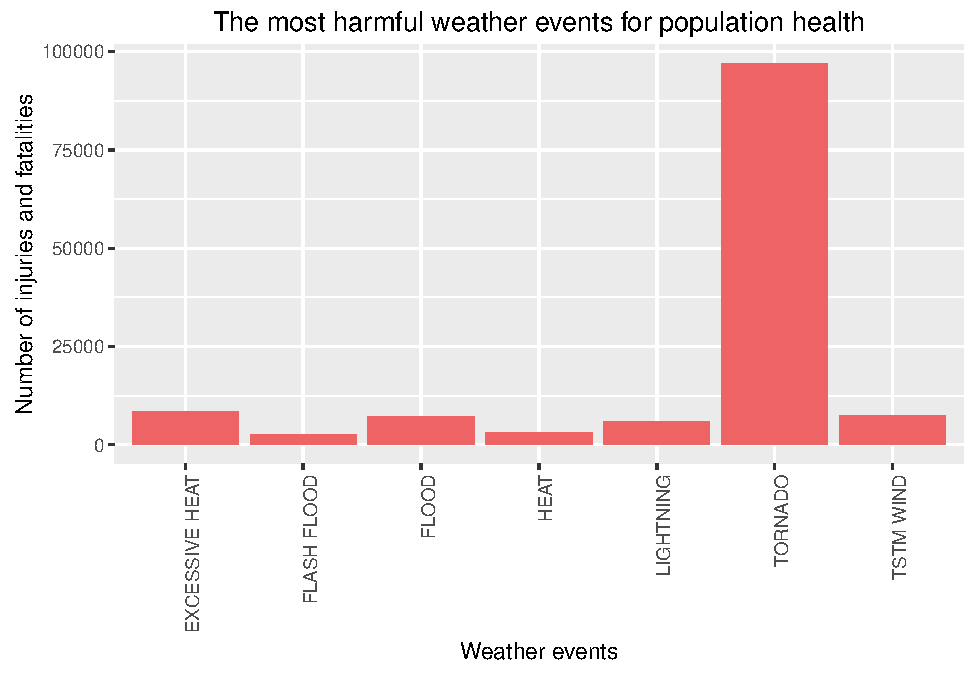
\includegraphics{HarmfulEvents_files/figure-latex/unnamed-chunk-8-1.pdf}

\textbf{Answer:} The most harmful weather events for population health
is Tornado with 96979 victims.

\subsubsection{2.2 Question 2 - Across the United States, which types of
events have the greatest economic
consequences?}\label{question-2---across-the-united-states-which-types-of-events-have-the-greatest-economic-consequences}

\begin{Shaded}
\begin{Highlighting}[]
\KeywordTok{ggplot}\NormalTok{(}\DataTypeTok{data =} \KeywordTok{head}\NormalTok{(economicConsequences, }\DecValTok{7}\NormalTok{), }
       \KeywordTok{aes}\NormalTok{(}\DataTypeTok{x =} \KeywordTok{factor}\NormalTok{(EVTYPE), }
           \DataTypeTok{y =} \NormalTok{property_damage +}\StringTok{ }\NormalTok{crop_damage, }
           \DataTypeTok{fill =} \NormalTok{EVTYPE)) +}\StringTok{ }
\StringTok{  }\KeywordTok{geom_bar}\NormalTok{(}\DataTypeTok{stat=}\StringTok{"identity"}\NormalTok{, }
           \DataTypeTok{fill=}\StringTok{"#FFA54F"}\NormalTok{) +}\StringTok{ }
\StringTok{  }\KeywordTok{theme}\NormalTok{(}\DataTypeTok{axis.text.x =} \KeywordTok{element_text}\NormalTok{(}\DataTypeTok{angle =} \DecValTok{90}\NormalTok{, }
                                   \DataTypeTok{hjust =} \DecValTok{1}\NormalTok{)) +}\StringTok{ }
\StringTok{  }\KeywordTok{ggtitle}\NormalTok{(}\StringTok{"Weather events with the highest economic consequences"}\NormalTok{) +}\StringTok{ }
\StringTok{  }\KeywordTok{xlab}\NormalTok{(}\StringTok{"Weather events"}\NormalTok{) +}\StringTok{ }
\StringTok{  }\KeywordTok{ylab}\NormalTok{(}\StringTok{"Total damage in $"}\NormalTok{)}
\end{Highlighting}
\end{Shaded}

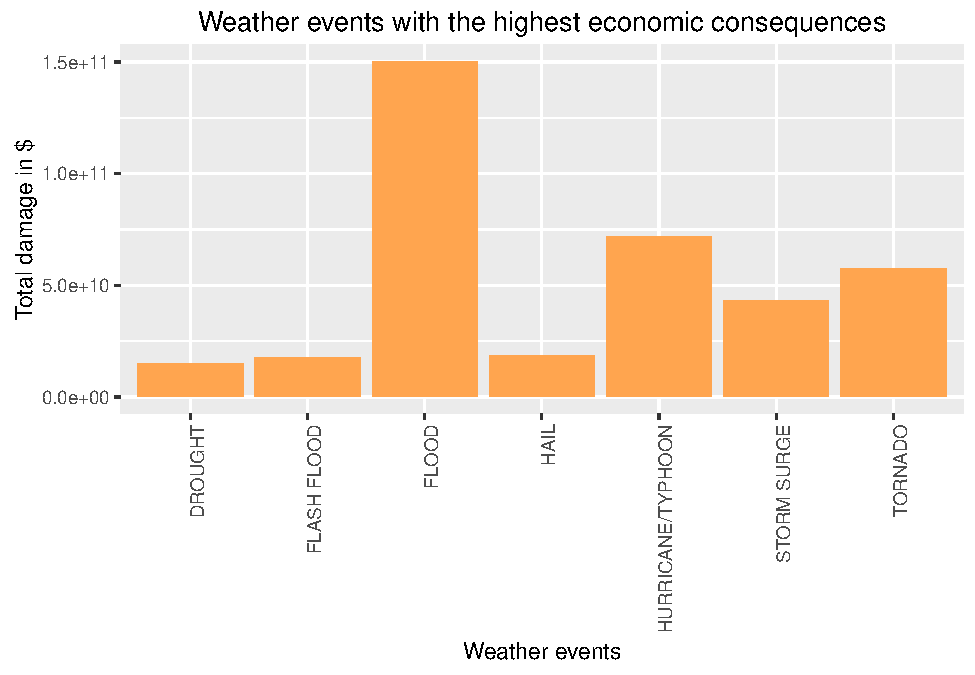
\includegraphics{HarmfulEvents_files/figure-latex/unnamed-chunk-9-1.pdf}

\textbf{Answer:} Event with the highest economic consequences is Flood
with 5661968450 \$ damage.

\end{document}
